\documentclass[conference]{IEEEtran}
\usepackage{blindtext, graphicx}
\usepackage{amsmath}
\usepackage{listings}
\usepackage{booktabs}
\usepackage{multirow}
\usepackage{tabularx}

\ifCLASSINFOpdf
\else
\fi


% correct bad hyphenation here
\hyphenation{op-tical net-works semi-conduc-tor}


\begin{document}

% figures: only your own research
% paraphrases
% clearer statements related to the findings

\title{Redesigning CHIML: Orchestration Language for Chimera-Framework}

\author{\IEEEauthorblockN{Go Frendi Gunawan}
\IEEEauthorblockA{STIKI Malang\\ Malang, Indonesia\\
Email: frendi@stiki.ac.id}
\and
\IEEEauthorblockN{Jozua Ferjanus Palandi}
\IEEEauthorblockA{STIKI Malang\\
Malang, Indonesia\\
Email: jozuafp@stiki.ac.id}
\and
\IEEEauthorblockN{Subari}
\IEEEauthorblockA{STIKI Malang\\
Malang, Indonesia\\
Email: subari@stiki.ac.id}}


% make the title area
\maketitle


\begin{abstract}
%\boldmath
Component Based Software Engineering (CBSE) has been proven to be quite effective to deal with software complexity. Nowadays developers prefer to build micro-services rather than single monolithic application. Several SOA (Service Oriented Architecture) approaches like HTTP/REST API, CORBA, and BPEL are commonly used by developers. Some of those solutions are built under assumptions that the developers are either building the services from scratch or able to create abstraction layer for the pre-existing services. In most cases the assumptions are true. However there are cases when developers prefer to keep the architecture as simple as possible without any need to build additional abstraction layers. For example, when they work with mini-embeded system.

Previously, a YAML based orchestration language was developed for Chimera-Framework (A language agnostic framework for stand-alone and distributed computing). In this paper, we refine the orchestration language in order to let developers accessing pre-existing services without any need to build another abstraction layer.
\end{abstract}

% Note that keywords are not normally used for peerreview papers.
\begin{IEEEkeywords}
Chimera, CBSE, Orchestration Language
\end{IEEEkeywords}

\IEEEpeerreviewmaketitle

\section{Introduction}

Software development is a very interesting topic. The way people developing softwares is changing as new paradigms emerged. In turns, software development also affecting the culture. It change how people interact to each others as well as how they interact with computers.

As software become more and more complex, building and maintaining softwares is also become harder. Various approaches have been attempted in order to make the processes easier.

\section{Research Question}

In order to have a clear direction in our research, we are focusing in these two questions:

\begin{itemize}
    \item How to make a readable, compact, and intuitive orchestration language for Chimera-Framework.
    \item How the orchestration language compared to other possible solutions.
\end{itemize}

\section{Literature Survey}

\subsection{Orchestration and Choreography}

\subsection{SOA and Micro-service}

\subsection{HTTP/REST API}

\subsection{SOAP}

\subsection{CORBA, BPEL, and EJB}

\section{CHIML}

\subsection{Design}

{\lt CHIML} is a superset of `YAML`. So, any valid `YAML` is also a valid `CHIML`. And as `YAML` itself is a superset of `JSON`, any valid `JSON` is also a valid `CHIML`

\subsection{Semantic (Backus Naur Form)}

\begin{lstlisting}[caption=CHIML Semantic, label=chimlSemantic, language=bash, basicstyle=\small, breaklines=true]
<program> ::= <completeVars>
              <completeVerbose>
              <command>
              <completeCatch>
              <completeThrow>

<command> ::= <completeCommand>
            | <shortCommand>

<completeCommand> ::= <completeIns>
                      <completeOut>
                      <completeIf>
                      "do: "<singleCommand><newLine>
                      <completeWhile>

                    | <completeIns>
                      <completeOut>
                      <completeIf>
                      "parallel: "<singleCommand><newLine>
                      <completeWhile>

                    | <completeIns>
                      <completeOut>
                      <completeIf>
                      "do: "<commandList>
                      <completeWhile>

                    | <completeIns>
                      <completeOut>
                      <completeIf>
                      "parallel: "<commandList>
                      <completeWhile>

                    | "map: "<variableName>
                      "into: "<variableName>
                      <completeCommand>

                    | "filter: "<variableName>
                      "into: "<variableName>
                      <completeCommand>

<shortCommand> ::= "|("<ins>") -> " <singleCommand> " -> " <out><newLine>
                 | "|("<ins>") -> " <singleCommand> "<newLine>
                 | "|"<singleCommand> " -> " <out><newLine>
                 | "|("<ins>") --> " <out><newLine>
                 | "|"<out> " <-- ("<ins>")"<newLine>

<commandList>  ::= "- "<command>
                 | <commandList><commandList>

<completeCatch> ::= "" 
                  | "catch: "<condition><newLine>

<completeThrow> ::= ""
                  | "throw: "<string><newLine>

<completeVars>  ::= ""
                  | "vars: "<variableList><newLine>

<completeVerbose> ::= ""
                    | "verbose: "<verbosity><newLine>

<completeIns>   ::= ""
                  | "ins: "<ins><newLine>

<completeOut>   ::= ""
                  | "out: "<out><newLine>

<completeIf>    ::= ""
                  | "if: "<condition><newLine>

<completeWhile> ::= ""
                  | "While: "<condition><newLine>

<ins> ::= <variableList>

<out> ::= <variableName>

<singleCommand> ::= <cliCommand>
                  | <jsArrowFunction>
                  | "{"<jsNormalFunction>"}"
                  | "["<jsFunctionWithCallback>"]"
                  | "<"<jsPromise>">"

<variableName> ::= <alpha>
                 | <alpha><alphaNumeric>

<variableList> ::= <variableName>
                 | <variableName>","<variableList>

<float> ::= <integer>
          | <integer>"."<integer>

<verbosity> ::= "1"
              | "2"
              | "3"
              | "4"

<condition> ::= "true"
              | "false"
              | Any JavaScript statement evaluated to either "true" or "false"

<string> ::= <string><string>
           | <alphanumeric>
           | <space>
           | <symbol>

<alphanumeric> ::= <alphanumeric><alphanumeric>
                 | <alpha>
                 | <integer>

<alpha> ::= <letter><alpha>

<letter> ::= single character, a-z or A-Z

<space> ::= " "

<newLine> ::= "\n"

<symbol> ::= single non-letter and non-numeric character

<integer> ::= <digit>
            | <digit><integer>

<digit> ::= "0" | "1" | "2" | "3" | "4" | "5" | "6" | "7" | "8" | "9"

<cliCommand> ::= Any valid CLI command

<jsArrowFunction> ::= Javascript arrow function

<jsNormalFunction> ::= Javascript function returning a value

<jsFunctionWithCallback> ::= Javascript function that has error-first-callback

<jsPromise> ::= Javascript promise
\end{lstlisting}

\subsection{Default Variables}

\subsection{Implementation}

\section{Experiment}

\subsection{Solutions}

\section{Result and Discussion}


\begin{figure}
	\centering
	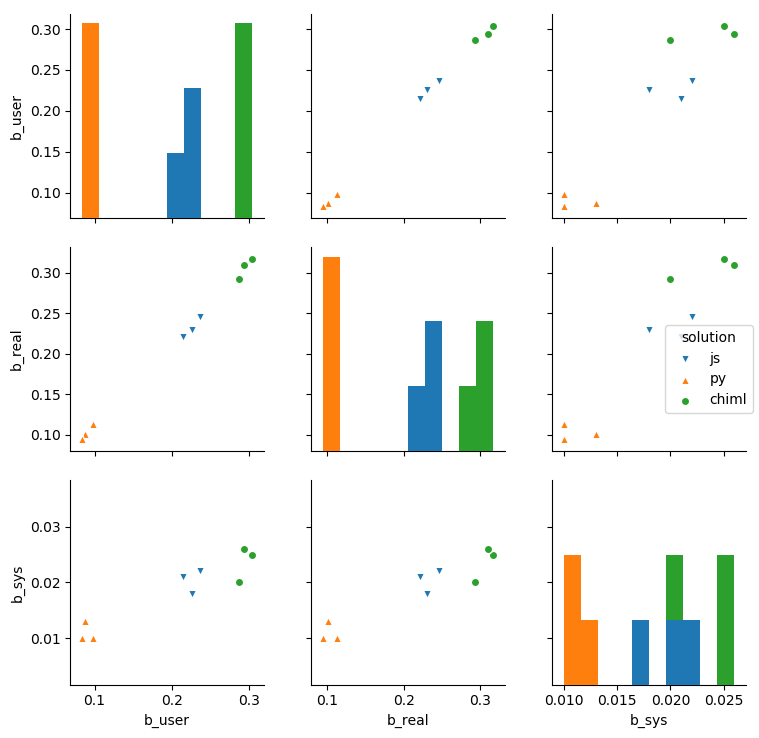
\includegraphics[width=0.3\textwidth]
		{benchmark/benchmark.png}
	\caption{Performance Comparison}
	\label{fig:performanceComparison}
\end{figure}


\begin{figure}
	\centering
	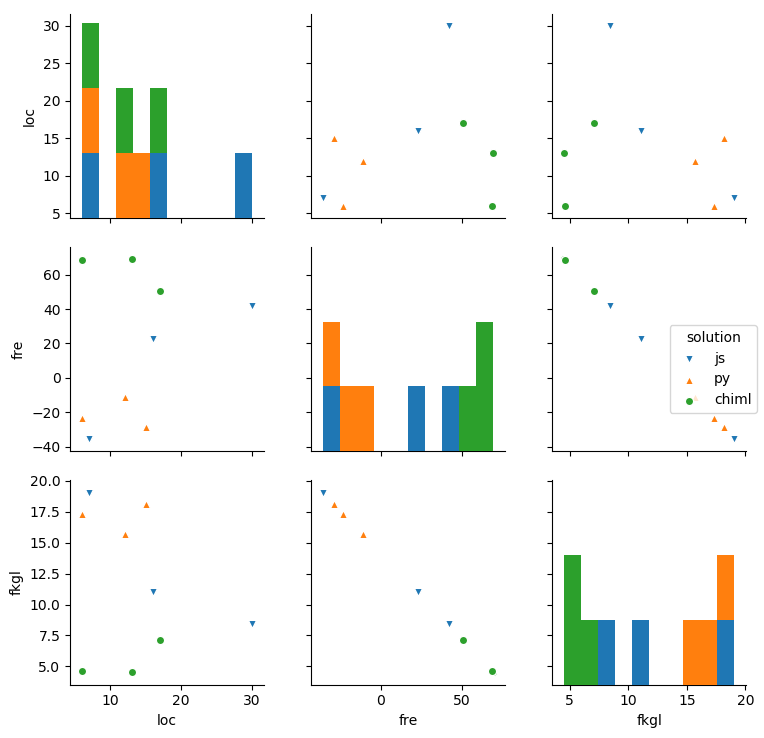
\includegraphics[width=0.3\textwidth]
		{benchmark/readability.png}
	\caption{Readability Comparison}
	\label{fig:readabilityComparison}
\end{figure}

\section{Conclusion}

CHIML serve well as orchestration language. However for control structure, the existance of intermediary components can help to boost performance. The best trait of CHIML is it's support for programming-in-large and programming-in-small. Eventough the control structure is still suffering for speed and performance, it serves well as prototyping tool. This mean that the developer can start orchestration solution in CHIML, then gradually do optimization.

%\appendices
%\section{Proof of the First Zonklar Equation}

% use section* for acknowledgement
\section*{Acknowledgment}

The authors would like to thank Sonny Setiawan, Satriyo Wibowo, Dani Devito, and Zusana Pudyastuti for their suggestions and inputs.

% Can use something like this to put references on a page
% by themselves when using endfloat and the captionsoff option.
\ifCLASSOPTIONcaptionsoff
  \newpage
\fi

\bibliographystyle{IEEEtran}
\bibliography{./citation}

% that's all folks
\end{document}

